\Task

Пусть нам задана монотонная функция $f(x)$
и какое-то значение $C$ этой функции. Необходимо найти значение аргумента $x$ этой функции, такое, что $f(x)\,=\,C$. 

\begin{figure}[h]
    \centering
    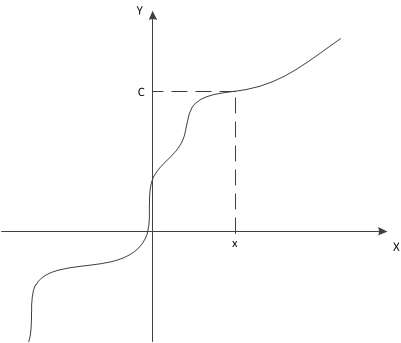
\includegraphics[width=0.3\linewidth]{pix/binsearch.png}
\end{figure}

\subsection*{Алгоритм}

Применим идею двоичного поиска. Выберем такие границы, где значение функции точно больше и точно меньше заданного значения. Выберем значение в середине этого отрезка. Если оно меньше, чем заданное, то сместим левую границу в середину отрезка. В противном случае сместим правую границу.

Есть несколько способов закончить поиск. К примеру, когда концы отрезка различается менее, чем на заданную погрешность $\varepsilon$.

\textit{Асимптотика.} $O\left(\log\left(\frac{r - l}{\epsilon}\right)\right)$.\\
\Proof\\
Мы знаем, что асимптотика целочисленного бинарного поиска - это $O(log\,n)$, где $n$ - длина промежутка, на котором запускается поиск. По сути, длина - это кол-во точек, в которых может оказаться искомое значение. Давайте узнаем "длину" для вещественного поиска. Искомая точка может оказаться в промежутках:
$\{[l, l + \epsilon), [l + \epsilon, l + 2\epsilon), \ldots\}$, то есть таких точек $\frac{r - l}{\epsilon}$ (Так как $\epsilon$ - это длина одного отрезка). А значит асимптотика вещественного бинарного поиска - $O\brackets{\log \brackets{\frac{r - l}{\epsilon}}}$. \Endproof
% \textit{Асимптотика.} $O\left(\frac{\log(r - l)}{\varepsilon}\right)$

\textbf{Псевдокод}

\begin{lstlisting}
double BinSearch(C: double) {
  left = findLeftBoard(C)
  right = findRightBoard(C)
  while (right - left > eps) {
    mid = (left + right) / 2
    if f(mid) < C {
      left = mid
    } else {
      right = mid
    }     
  }
  return (left + right) / 2
}
\end{lstlisting}
Источник: \href{https://neerc.ifmo.ru/wiki/index.php?title=Вещественный_двоичный_поиск}{Вещественный двоичный поиск}

\pagebreak